%!TeX program = xelatex
%Do not change
\documentclass[12pt, oneside]{article}
\usepackage{amssymb,amsmath}
\usepackage[margin=1in]{geometry}
\usepackage{textpos}
\usepackage{float}
\usepackage{booktabs}
%\usepackage{color}
\usepackage{graphicx}
\usepackage[inter-unit-product =\cdot]{siunitx}
\let\DeclareUSUnit\DeclareSIUnit
\let\US\SI
\DeclareUSUnit\inch{in}
\DeclareUSUnit\foot{ft}
\DeclareUSUnit\mile{mi}
\DeclareUSUnit\foot{ft}
\DeclareUSUnit\slug{slug}
\DeclareUSUnit\pound{lb}
\DeclareUSUnit\psi{psi}
\DeclareUSUnit\Msi{Msi}
\DeclareUSUnit\ksi{ksi}

%\usepackage{tikz}
%\usetikzlibrary{positioning}
%\usepackage{tikz-3dplot}
%\usepackage{pgfopts}
%\usepackage{wasysym}
%\usepackage{stanli}

% You may add the packages you need here
\begin{document}

%TODO change numbers in problems
\begin{textblock*}{4cm}(-1.7cm,-2.3cm)
\noindent {\scriptsize AE333 Spring 2021}
\end{textblock*}

%Do not modify other than putting your name where stated
\begin{textblock*}{8cm}(12.5cm,-1cm)
\noindent {Name: }
\end{textblock*}
%Do not modify other than typing your acknowledgement where stated
\begin{textblock*}{13.5cm}(-1.7cm,-1.8cm)
%\noindent \textit{\footnotesize Acknowledgement: Your acknowledgement for collaboration and other sources goes here. }
\end{textblock*}

\vspace{1cm}

%Do not modify other than typing the homework number after #
\begin{center}
\textbf{\Large Homework 6 Solutions}

\textbf{Due 5 April 2021}
\end{center}

\begin{enumerate}
	\item %F7-2
		Find the shear stress at points $A$ and $B$ when $V = 	\SI{450}{kN} $.
		Draw the state of stress on a volume element at each point.
		\begin{figure}[H]
			\centering
			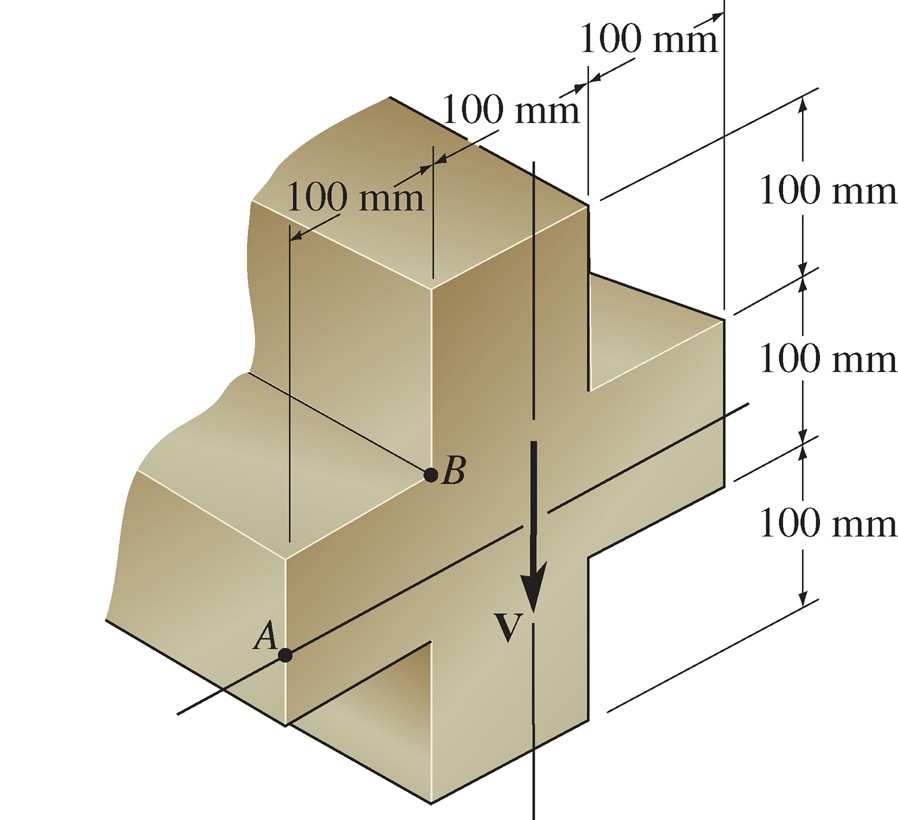
\includegraphics[width=0.6\linewidth]{f7-2}
		\end{figure}
			\textbf{Solution:}
			\begin{itemize}
				\item Since we are given $V$, we just need to find $Q$, $I$, and $t$ at each point
				\item There are several ways to go about calculating $I$, I will use a method that might seem counter-intuitive.
					I will consider the two rectangles shown in red and blue (which overlap), and then subtract the overlapping square (but only once).
					Another alternative would be to calculate one rectangle and then add the two squares left over (note that this way requires using the parallel axis theorem).
					\begin{figure}[H]
						\centering
						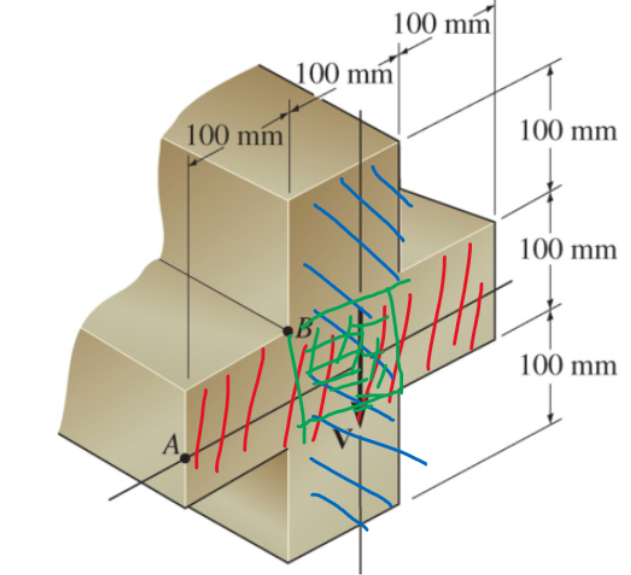
\includegraphics[width=0.6\linewidth]{6-1a}
					\end{figure}
				\item This gives $I= 	\SI{2.42e8}{mm^4} $Note: since this section is symmetric, the neutral axis (centroid) is in the center and all our inertias reference that
				\item To find $Q$ we find the area above points $A$ and $B$ respectively, we find $A^\prime_B = 	\SI{1e4}{mm^2} $, $A^\prime_A = 	\SI{2.5e4}{mm^2} $, $\bar{y}^\prime_B = 	\SI{100}{mm} $ and $\bar{y}^\prime_A = 	\SI{55}{mm} $ which gives $Q_B = 	\SI{1e6}{mm^3} $ and $Q_A = 	\SI{1.375e6}{mm^3} $
				\item $t$ can be found from the geometry with $t_b = 	\SI{100 }{mm} $ and $t_a = 	\SI{300}{mm} $
				\item This gives $\tau_B = 	\SI{18.6 }{MPa} $ and $\tau_A = 	\SI{8.53}{MPa} $ and the stress state on representative volume elements looks like:
					\begin{figure}[H]
						\centering
						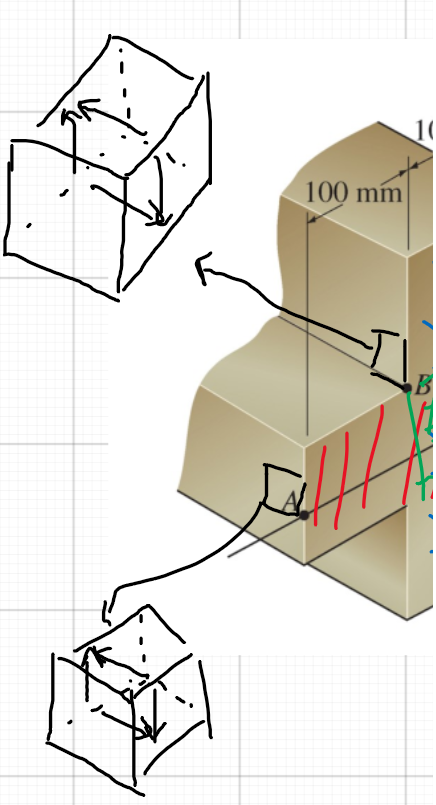
\includegraphics[width=0.2\linewidth]{6-1b}
					\end{figure}
			\end{itemize}

	\item %7-25
		Find the maximum shear stress acting on the beam shown.
		\begin{figure}[H]
			\centering
			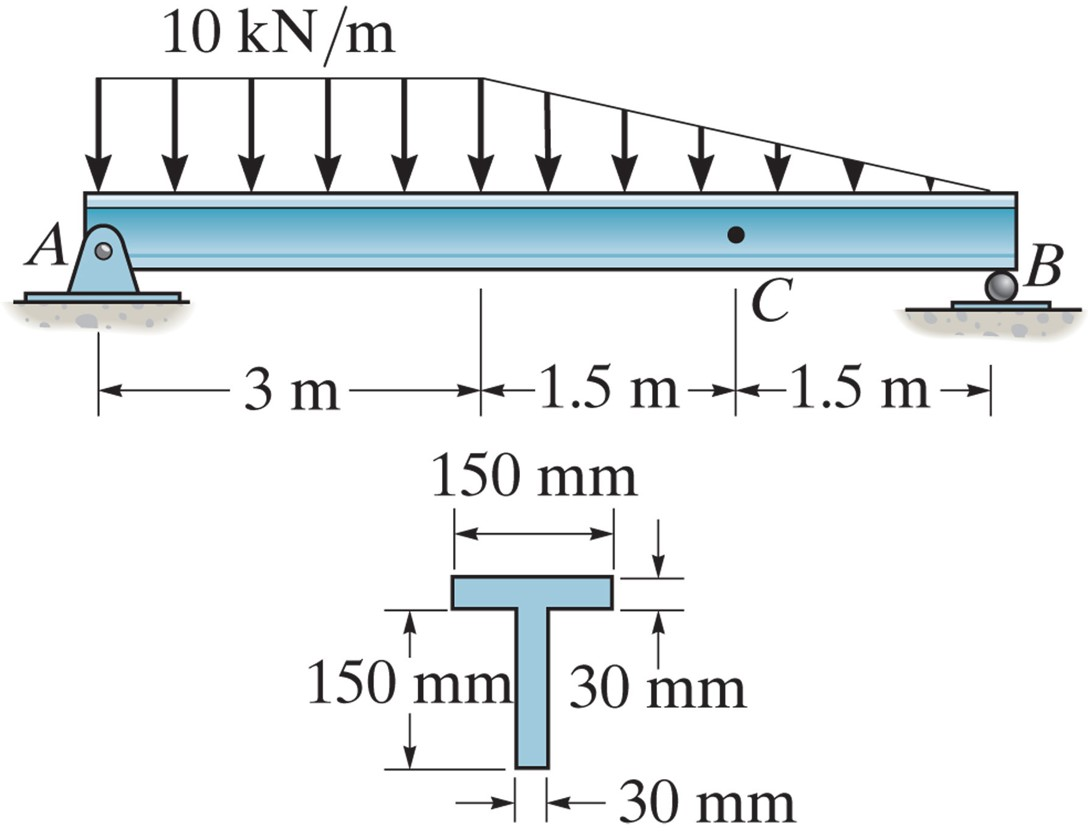
\includegraphics[width=0.6\linewidth]{7-25}
		\end{figure}
			\textbf{Solution:}
			\begin{itemize}
				\item We start with a free body diagram and a shear diagram
					\begin{figure}[H]
						\centering
						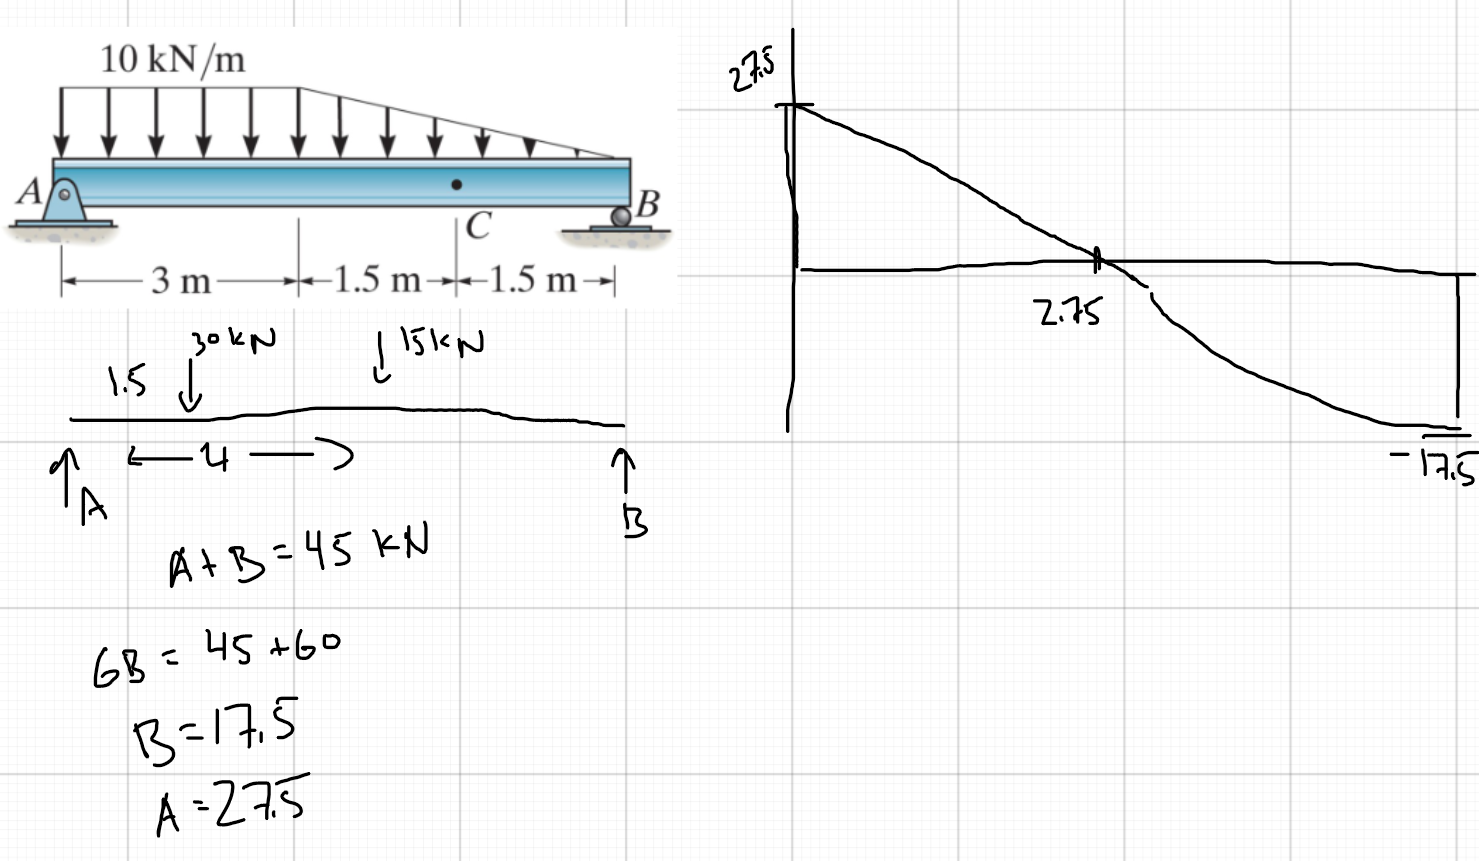
\includegraphics[width=0.8\linewidth]{6-2}
					\end{figure}
				\item We see that the maximum shear force is $ \SI{27.5 }{kN} $, so now we find $I$, $Q$, and $t$
				\item This cross-section is not symmetric, so we begin by finding the neutral axis $\bar{y} = \frac{(75)(30)(150)+(165)(150)(30)}{2(150)(30)} = 	\SI{120}{mm} $ (measured from the bottom)
				\item Next we find the inertia, $I = \frac{1}{12}(30)(150^3) + (30)(150)(75-120)^2 + \frac{1}{12}(150)(30^3) + (150)(30)(120-75)^2 = 	\SI{2.7e7}{mm^4} $
				\item Typically, the maximum shear stress occurs at the center (unless there is a thin section far away from the center, as occurred in problem 1), since the thinnest region is at the center, we expect the maximum shear to occur at the center, and we calculate $Q$ there.
					We can find $Q$ by considering the area either above or below the point, and in this case the area below is much easier.
					$Q = (30)(120)(120-60) = 	\SI{2.16e5}{mm^3} $
				\item Finally, we use $t= 	\SI{30 }{mm} $ to calculate the shear stress as $ 	\SI{7.33}{MPa}  $
			\end{itemize}

	\item %7-11
		The overhanging beam is subjected to a uniform load of $w= 	\SI{75}{kN/m} $.
		Find the maximum shear stress in the beam.
		\begin{figure}[H]
			\centering
			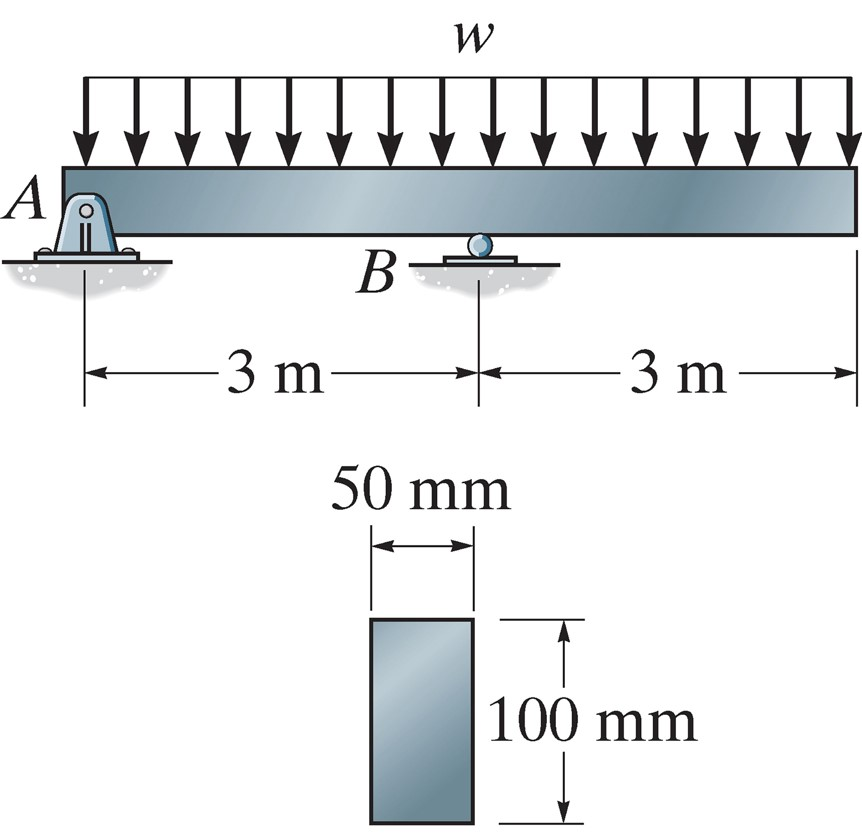
\includegraphics[width=0.5\linewidth]{7-11}
		\end{figure}
		\textbf{Solution:}
		\begin{itemize}
			\item From statics analysis, we find the reaction force at $A$ is 0 and the maximum shear force of $V = \SI{225}{kN}$ occurs at $B$
			\item Next we find $I = \frac{1}{12}bh^3 = \frac{1}{12}50(100^3) = \SI{4.17e6}{mm^4}$
			\item Since this is a solid rectangular cross-section, the maximum shear will occur at the middle and we can find $Q = \bar{y}^\prime A^\prime = (25)(50)(50) = \SI{6.25e4}{mm^3}$
			\item We can now find the maximum shear stress $\tau = \frac{VQ}{IT} = \SI{67.5 }{MPa}$
		\end{itemize}

	\item %F7-7
		Two identical $ 	\SI{20 }{mm}  $ plates are bolted to the top and bottom of a flange to form a built-up beam.
		For a shear force of $V = 	\SI{400 }{kN} $ find the maximum bolt spacing, $s$, if each bolt has a shear strength of $ 	\SI{45 }{kN}  $
		\begin{figure}[H]
			\centering
			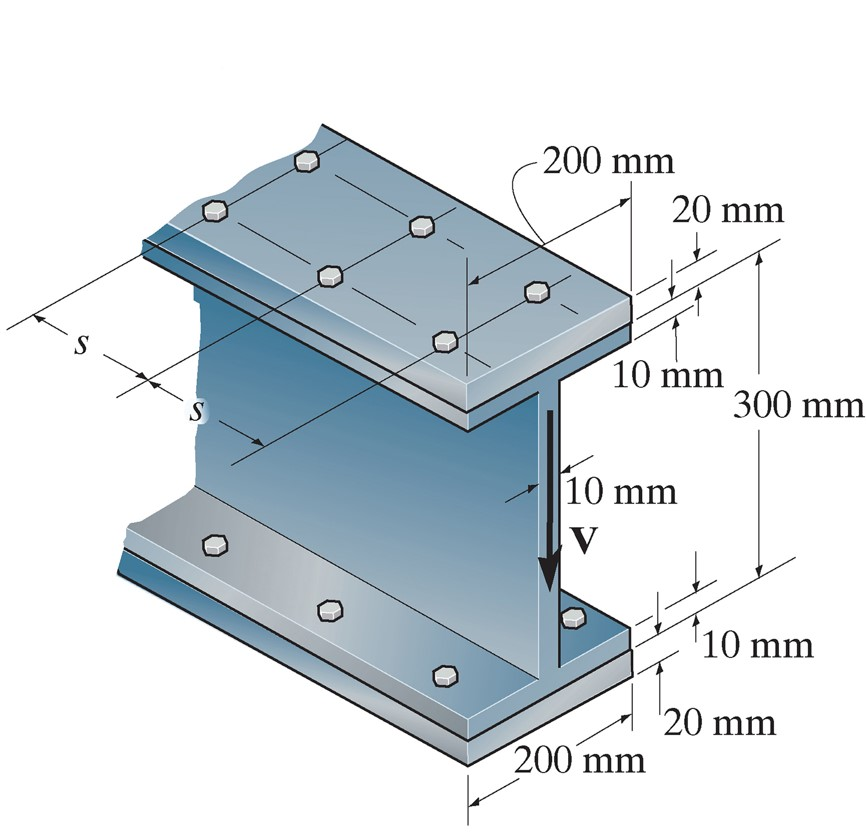
\includegraphics[width=0.6\linewidth]{f7-7}
		\end{figure}
		\textbf{Solution:}
		\begin{itemize}
			\item We start by calculating the inertia of the entire cross-section, since this is needed to find the shear flow, $q$
			\item $I = \frac{1}{12}(10)(280^3) + 2\left[ \frac{1}{12}(200)(30^3) + (200)(30)(155^2) \right] = \SI{3.075e8}{mm^4}$
			\item Next we need to find the moment of area, $Q$, for the area to be bolted on $Q = \bar{y}^\prime A^\prime = (160)(20)(200) = \SI{6.4e5}{mm^3}$
			\item We can now solve for the shear flow, $q = \frac{VQ}{I} = \SI{833}{N/mm}$
			\item Next we use $F = qs$ to solve for the spacing with $F= \SI{45 }{kN}$ and we find $s=\SI{54.1 }{mm}$
		\end{itemize}

	\item %7-46
		The beam shown is made by gluing two $ 	\US{1/2 }{in}  $ c-channel strips together as sown.
		If the glue has a maximum shear stress of $\tau = 	\US{600}{psi} $ find the maximum intensity, $w_0$, of the triangular distributed loading.
		\begin{figure}[H]
			\centering
			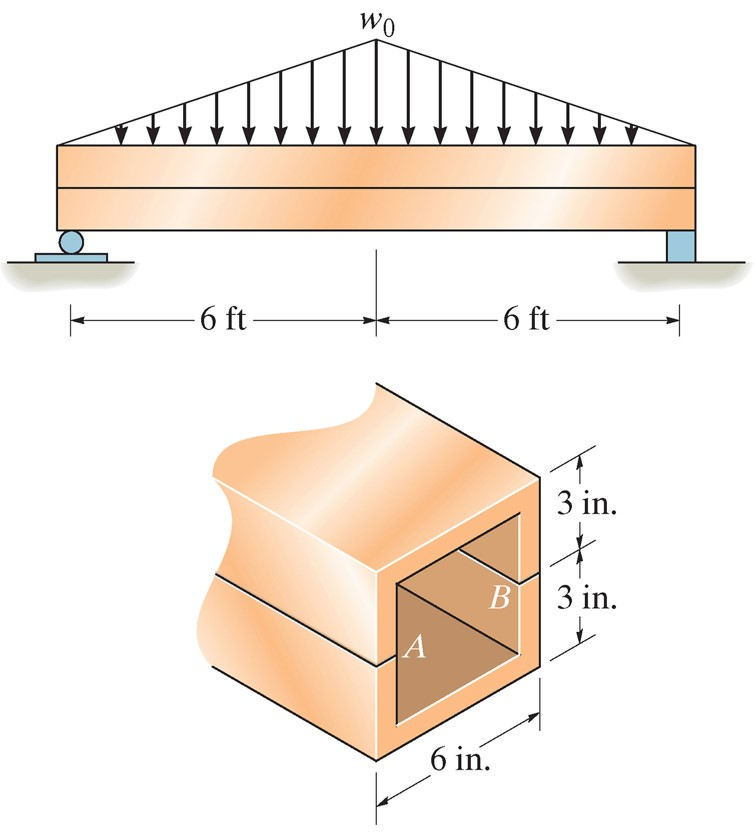
\includegraphics[width=0.6\linewidth]{7-46}
		\end{figure}
		\textbf{Solution:}
		\begin{itemize}
			\item Since this is symmetric we can quickly see that the highest shear force will occur at each support and is equal to $V = w_0 6 / 4$
			\item The easiest way to find the inertia is to consider the tube to be solid and subtract the inside $ I = \frac{1}{12} (6)(6^3) - \frac{1}{12}(5)(5^3) = \US{55.9}{in^4} $
			\item $Q$ can be found in the same fashion, by considering the entire top half (as if it were solid) and subtracting the empty space, $Q = (6)(3)(1.5) - (5)(2.5)(1.25) = \US{11.4}{in^3}$
			\item Finally we find $t = 2(0.5) = \US{1}{in}$ and we can solve $\tau = \frac{VQ}{It}$ for $w_0$ (note that we need to convert length units to all be in inches) to find $w_0 = \US{164}{lb/in} = \US{1.97}{kip/ft}$
		\end{itemize}

\end{enumerate}
\end{document}
